\newcommand{\usecasefigure}[2]{
	\begin{figure}[htp]
		\centering
		\includegraphics[width=0.8\textwidth]{images/useCases/#1.png}
		\caption{Use case diagram #2}
		\label{fig:use_cases_#1}
	\end{figure}
	\newpage
}

This section contains all the use cases initially described with the use case UML models, then the most important Use Cases have their own table which provides further details such as: involved actors, entry conditions, flow of events,  exit conditions and exceptional conditions.

\subsubsection{User Page use cases}
\begin{figure}[htp]
	\centering
	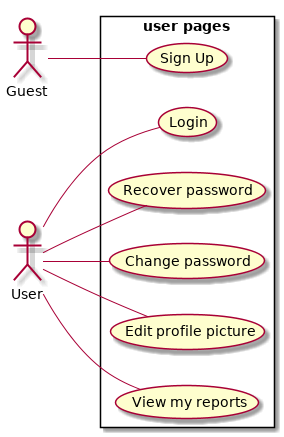
\includegraphics[width=0.6\textwidth]{images/useCases/uc_user_page.png}
	\caption{Use cases relative to the user registration and authentication} 
	\label{fig:userpage} 
\end{figure} 

\newpage
\begin{enumerate}
	\item \textbf{Sign Up}\\
		\begin{table}[!htbp]
\centering
\begin{tabular}{lp{8cm}}
\bf\large Name&\bf\large Sign up\\
\hline
\hline
\bf Actors&Guest\\
\hline
\bf Entry conditions&None\\
\hline
\bf Flow of events&
\begin{itemize}
\item The guest reaches the registration page containing the relative form
\item The guest fills up the form and clicks on "Sign up" to complete the process
\item The system redirects the user to his profile page.
\end{itemize}
\\
\hline
\bf Exit conditions&The guest has successfully registered into SafeStreets. \\
\hline
\bf Exceptions&The guest left an empty field or typed
 something invalid: an error message is displayed 
 and the user is asked to fill the form again.\\
\hline

\end{tabular}
\caption{Use Case table - Sign up} \label{tab:signup}
\end{table}

		\newpage
		\textbf{Diagrams}
		\usecasefigure{sign_up}{of the signup process}
		\newpage
	\item \textbf{Login}\\
		\begin{table}[!htbp]
\centering
\begin{tabular}{lp{8cm}}
\bf\large Name&\bf\large Login\\
\hline
\hline
\bf Actors&User\\
\hline
\bf Entry conditions&The user had already registered in the past.\\
\hline
\bf Flow of events&
\begin{itemize}
\item The user reaches the login page containing the relative form
\item The user types the username and password in the login form and clicks on the "Login" button.
\item The system redirects the user to the application homepage.
\end{itemize}
\\
\hline
\bf Exit conditions&The user has access to the application functionalities. \\
\hline
\bf Exceptions&Username and password didn't correspond or the username didn't exist: an error message is displayed and the user is asked to fill the login form again.\\
\hline

\end{tabular}

\caption{Login Use Case table} \label{tab:login}
\end{table}
		\newpage
		\textbf{Diagrams}
		\usecasefigure{login}{of the login process}
		\newpage
	\item \textbf{Password Recovery}\\
		\begin{table}[!htbp]
	
	\hypertarget{tab:recoverpasswordusecase}{}
	\centering
	\begin{tabular}{lp{8cm}}
		\bf\large Name&\bf\large Recover Password \\
		\hline
		\hline
		\bf Actors&User\\
		\hline
		\bf Entry conditions&The user had already registered in the past.\\
		\hline
		\bf Flow of events&
		\begin{itemize}
			\item The user reaches the login page containing the relative form
			\item The user does not remember his password so he clicks on "Password recovery" button and is redirected to the password recovery page.
			\item The user inserts his email and clicks on "reset password".
			\item The system sends an email to the user with a link and instruction to reset the password.
			\item The user chooses and types a new password and confirms.
			\item The system redirects the user to the login page.
		\end{itemize}
		\\
		\hline
		\bf Exit conditions&The user requested an email to reset his password \\
		\hline
		\bf Exceptions&The inserted email does not match any user in the database, it is displayed an error message and the user is asked to retype a valid email.\\
		\hline
		
	\end{tabular}
	\caption{Recover password Use Case table} \label{tab:recoverpassword}
\end{table}
		\newpage
		\textbf{Diagrams}
		\usecasefigure{password_recovery}{of the password recovery process}
		\newpage
\end{enumerate}
\newpage

\subsubsection{Report and Information Management use cases}
\begin{figure}[htp]
	\centering
	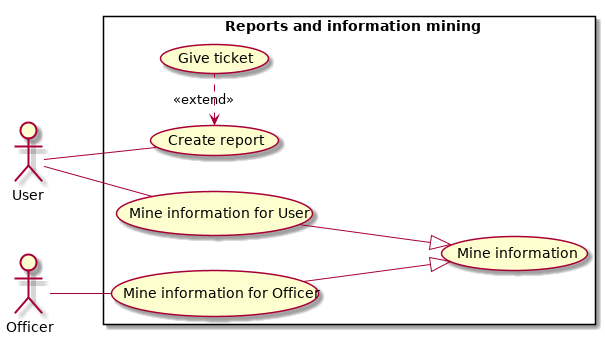
\includegraphics[width=\textwidth]{images/useCases/uc_report_and_information_mining.png}
	\caption{Main use cases showing the functionalities of SafeStreets application relative to the user report management and information mining.} 
	\label{fig:reportmanagement} 
\end{figure}

\newpage
\begin{enumerate}
	\setcounter{enumi}{3}
	\item \textbf{Report Creation}\\
		\begin{table}[!htbp]
	\centering
	\begin{tabular}{lp{9cm}}
\bf\large Name&\bf\large Creation of a new report\\
\hline
\hline
\bf Actors&User\\
\hline
\bf Entry conditions&The user is logged in and is in the main page.\\
\hline
\bf Flow of events&
\begin{itemize}

\item The user clicks on "Report Violation" button and is redirected to the page with the input form to create a new report.

\item The user fills up the form with the violation information (type of violation, pictures of it, address, description, license plate position, date and time, etc...). Eventually some fields such as date and time will be auto-completed.

\item The user clicks on the "Send Report" button after a quick check of all the field he typed.

\item The system show the user a confirmation message. 

\item The user is then redirected to the main page.

\end{itemize}
\\
\hline
\bf Exit conditions&The new report with the user-inserted data is created into the SafeStreets system. In the case of the violation to result in a duplicate (possibly by another user) of in case of the license plate to be not readable, the system put this report in a revision queue and block the process.\\
\hline
\bf Exceptions&The information inserted is wrong (non-existent address, date and time in the future) or some information is missing: a corresponding error is displayed and the user is asked to modify the inserted information accordingly.
\\
\hline

\end{tabular}
\caption{Report Creation Use Case table}
 \label{tab:reportcreationtab}
\end{table}
		\newpage
		\textbf{Diagrams}
		\usecasefigure{creation_of_new_report}{of the report creation process}
		\newpage
	\item \textbf{Automatic Traffic Ticket generation}\\
		\begin{table}[!htbp]
	\hypertarget{tab:AutomaticTrafficTicket}{}
	\centering
	\begin{tabular}{lp{10cm}}
\bf\large Name&\bf\large Automatic Traffic Ticket generation\\
\hline
\hline
\bf Actors&User\\
\hline
\bf Entry conditions&The user is logged in and is in the main page.\\
\hline
\bf Flow of events&
\begin{itemize}
\itemsep0em 
\item The user clicks on "Report Violation" button and is redirected to the input form to create a report.

\item The user fills up the form with the violation information (type of violation, pictures of it, address, description, license plate position, date and time, etc...). Eventually some fields such as date and time will be auto-completed.

\item The user clicks on the "Verified Violation" checkbox because he is sure of it being a violation because it's evident or any other motivation.

\item The user clicks on the "Send Report" button after a quick check of all the field he typed.

\item The system shows a confirmation message to the user and redirects him to the main page.

\end{itemize}
\\
\hline
\bf Exit conditions&The new report is created into the SafeStreets system and passed to the Local Police service.\\
\hline
\bf Exceptions&
\setlist{nolistsep}
\begin{itemize}
	\itemsep0em 
	\item The information inserted is wrong (non-existent address, date and time in the future) or some information is missing: a corresponding error is displayed and the user is asked to modify the inserted information accordingly.
	\item The violation results in a duplicate or the license plate is not readable: the system put this report in a revision queue and block the process.
\end{itemize}
\\
\hline

\end{tabular}
\caption{Automatic Traffic Ticket generation Use Case table}
 \label{tab:AutomaticTrafficTicket}
\end{table}
		\newpage
		\textbf{Diagrams}
		\usecasefigure{automatic_traffic_ticket}{of the traffic ticket generation process}
		\newpage
	\item \textbf{Information Mining by Users (Unsafe Area)}\\
		\begin{table}[!htbp]
	\hypertarget{tab:dataminingtab}{}
	\centering
	\begin{tabular}{lp{9cm}}
\bf\large Name&\bf\large Information Mining by users\\
\hline
\hline
\bf Actors&User\\
\hline
\bf Entry conditions&The user is logged in and is in the main page.\\
\hline
\bf Flow of events&
\begin{itemize}

\item The user clicks on the "Unsafe Areas" button and is redirected to the page with the general SafeStreets statistics about various areas in the city.

\item The user clicks on the selection menu to choose which area he wants to see, possibly entering its name or an address in that area.

\item The user could analyze the data that will be shown with a practical map and the textual information.

\item After he finishes, he presses the Home button.

\item The user is then redirected to the main page.

\end{itemize}
\\
\hline
\bf Exit conditions&The user-requested analytics is displayed to the user at the level of aggregation he has chosen (these kind of information is not sensitive).\\
\hline
\bf Exceptions&The selected area is actually not present on SafeStreets or nonexistent: an error is displayed and he is asked to modify the inserted location accordingly.
\\
\hline

\end{tabular}
\caption{Data Mining Use Case table}
 \label{tab:dataminingtab}
\end{table}
		\newpage
		\textbf{Diagrams}
		\usecasefigure{information_mining}{of the information mining process (unsafe area) for a user}
		\newpage
	\item \textbf{Information Mining by Officers (Unsafe Area)}\\
		\begin{table}[!htbp]
	\hypertarget{tab:dataminingofficertab}{}
	\centering
	\begin{tabular}{lp{9cm}}
\bf\large Name&\bf\large Information Mining by officers\\
\hline
\hline
\bf Actors&Officer\\
\hline
\bf Entry conditions&The officer is logged in and is in the main page of his software.\\
\hline
\bf Flow of events&
\begin{itemize}

\item The officer clicks on the "Statistics" section button and is redirected to a page with the general SafeStreets statistics (such as number of usages, last use date, etc) in the officer municipality.

\item The officer clicks on the selection menu to switch between statistics related to his municipality, possibly exporting it in CSV (most dangerous areas, vehicles with highest frequency of violations, etc).

\item The officer could analyze the data that will be shown and after he finishes, he presses the Home button.

\item The officer is then redirected to the main page.

\end{itemize}
\\
\hline
\bf Exit conditions&The officer-requested analytics is displayed to the officer for the municipality land.\\
\hline
\bf Exceptions&None.
\\
\hline

\end{tabular}
\caption{Data Mining for Officers Use Case table}
 \label{tab:dataminingofficertab}
\end{table}
		\newpage
		\textbf{Diagrams}
		\usecasefigure{information_mining_by_officers}{of the information mining process (unsafe area) for an officer}
		\newpage
	\item \textbf{Information Mining by Users (Vehicle Violations)}\\
		\begin{table}[!htbp]
	\hypertarget{tab:dataminingvehicletab}{}
	\centering
	\begin{tabular}{lp{9cm}}
		\bf\large Name&\bf\large Information Mining by Users\\
		\hline
		\hline
		\bf Actors&User\\
		\hline
		\bf Entry conditions&The user is logged in and is in the main page.\\
		\hline
		\bf Flow of events&
		\begin{itemize}
			
			\item The user clicks on the "Worst Drivers" button and is redirected to the page with the general SafeStreets statistics about vehicle infractions in the city grouped by license plate.
			
			\item The user clicks on the calendar menu to choose which time frame he's interested in, possibly entering its more information such as the violation type.
			
			\item The user could analyze the data that will be shown in order of number of violations.
			
			\item After he finishes, he presses the Home button.
			
			\item The user is then redirected to the main page.
			
		\end{itemize}
		\\
		\hline
		\bf Exit conditions&The user-requested analytics is displayed to the user at the level of aggregation he has chosen (these kind of information is not sensitive).\\
		\hline
		\bf Exceptions&The inserted time frame is invalid: an error is displayed and he is asked to modify the desired time frame.
		\\
		\hline
		
	\end{tabular}
	\caption{Data Mining for Vehicle Use Case table}
	\label{tab:dataminingvehicletab}
\end{table}
		\newpage
		\textbf{Diagrams}
		\usecasefigure{information_mining_vehicle}{of the information mining process (vehicle violations) for an officer}
		\newpage
	\item \textbf{Information Mining by Officers (Vehicle Violations)}\\
		\begin{table}[!htbp]
	\hypertarget{tab:dataminingvehicleofficerstab}{}
	\centering
	\begin{tabular}{lp{9cm}}
		\bf\large Name&\bf\large Information Mining by officers\\
		\hline
		\hline
		\bf Actors&Officer\\
		\hline
		\bf Entry conditions&The officer is logged in and is in the main page of his software.\\
		\hline
		\bf Flow of events&
		\begin{itemize}
			
			\item The officer clicks on the "Worst Drivers" button and is redirected to the page with the general SafeStreets statistics about vehicle infractions in the officer municipality grouped by license plate.
			
			\item The officer clicks on the calendar menu to choose which time frame he's interested in, possibly entering its more information such as the violation type with the possibility to export it in CSV.
			
			\item The officer could analyze the data that will be shown in both textual and graphical form.
			
			\item After he finishes, he presses the Home button.
			
			\item The officer is then redirected to the main page.
			
		\end{itemize}
		\\
		\hline
		\bf Exit conditions&The officer-requested analytics is displayed to the officer for the municipality land.\\
		\hline
		\bf Exceptions&The inserted time frame is invalid: an error is displayed and the officer is asked to modify the desired time frame.
		\\
		\hline
		
	\end{tabular}
	\caption{Data Mining for Vehicle by Officers Use Case table}
	\label{tab:dataminingvehicleofficerstab}
\end{table}
		\newpage
		\textbf{Diagrams}
		\usecasefigure{mining_vehicle_officers}{of the information mining process (vehicle violations) for an officer}
		\newpage
\end{enumerate}
\newpage


\subsubsection{Statistics use cases}
\begin{figure}[htp]
	\centering
	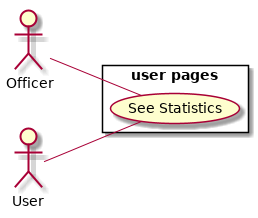
\includegraphics[width=\textwidth]{images/useCases/uc_statistics.png}
	\caption{Simple use case demonstrating the functionalities of SafeStreets application to provide statistics of its usage.} 
	\label{fig:statisticsuc} 
\end{figure}

\newpage
\begin{enumerate}
	\setcounter{enumi}{9}
	\item \textbf{Statistics and analytics consulting}\\
	\begin{table}[!htbp]
	\hypertarget{tab:statisticsconsultingtab}{}
	\centering
	\begin{tabular}{lp{9cm}}
		\bf\large Name&\bf\large Statistics and analytics consulting\\
		\hline
		\hline
		\bf Actors&Both Users or Officers\\
		\hline
		\bf Entry conditions&The actor is logged in and he is in the main page.\\
		\hline
		\bf Flow of events&
		\begin{itemize}
			
			\item The actor clicks on the "Statistics" button and is redirected to the page with alle the general SafeStreets statistics such as Tickets given, App usages, Effectiveness, Violation Types...
			
			\item The user clicks on the statistic he's interested in.
			
			\item The user could analyze the analytics provided and can compare different analytics to acquire knowledge about the SafeStreets project.
			
			\item After he finishes, he presses the Home button.
			
			\item The actor is then redirected to the main page.
			
		\end{itemize}
		\\
		\hline
		\bf Exit conditions&The actor-requested analytics is displayed to the user (these kind of information is not sensitive).\\
		\hline
		\bf Exceptions&None.
		\\
		\hline
		
	\end{tabular}
	\caption{Statistics consulting Use Case table}
	\label{tab:statisticsconsultingtab}
\end{table}
	\newpage
	\textbf{Diagrams}
	\usecasefigure{general_statistics}{for an actor examining statistics}
	\newpage
\end{enumerate}
\newpage

